\documentclass[10pt]{article}
\usepackage[T1]{fontenc}
\usepackage[utf8]{inputenc}
\usepackage{lmodern}
\usepackage[a4paper,margin=18mm]{geometry}
\usepackage{amsmath,amssymb}
\usepackage{graphicx}
\usepackage{booktabs,longtable,array,ragged2e,seqsplit}
\usepackage{microtype}
\usepackage[hidelinks]{hyperref}
\pdfinfoomitdate=1
\pdfsuppressptexinfo=-1
\pdftrailerid{<474f5244414e2d54484554412d46494e31><474f5244414e2d54484554412d46494e31>}
\hypersetup{pdftitle={Apparatus for Gordan's Ueber die Transformation der Thetafunctionen},pdfauthor={Critical-diplomatic edition},pdfsubject={Source topology, exclusions, critical notes, asset evidence, and QA}}
\pagestyle{plain}
\setlength{\parindent}{0pt}
\setlength{\parskip}{0.45em}
\newcommand{\unit}[1]{\texttt{#1}}
\newcommand{\noteid}[1]{\textbf{#1}}
\begin{document}
\small

\begin{center}
{\Large Apparatus}\\[0.4em]
{\large Paul Gordan, \textit{Ueber die Transformation der Thetafunctionen} (1863)}\\[0.35em]
{\normalsize Final repaired critical-diplomatic edition}
\end{center}

\section*{1. Editorial status and authority}

This apparatus accompanies two independent products: a German diplomatic transcription and a faithful English rendering. It is not a corrected mathematical edition. The German body preserves the printed wording, spelling, punctuation, and mathematical anomalies wherever the pixels are legible. The English body translates the prose while retaining the same mathematical readings. Clarifications and rejected inherited readings are confined to the numbered notes below.

The controlling witness is the 20-unit authority PDF with SHA-256
\begin{quote}\ttfamily\small
c9b744640aa68f448f432bd495c68129a108dd15f6480fdb725aad1b035f73aa
\end{quote}
The convenience page-image witnesses were checked against that PDF. The edition uses stable invisible destinations \texttt{source-PA01} through \texttt{source-PA20}; the TeX source exposes them as \verb|\sourceanchor{PAxx}|.

\section*{2. Exact source topology and disposition}

\renewcommand{\arraystretch}{1.12}
\begin{longtable}{>{\ttfamily}p{0.10\linewidth} >{\RaggedRight\arraybackslash}p{0.29\linewidth} >{\RaggedRight\arraybackslash}p{0.51\linewidth}}
\toprule
Unit & Witness role & Scholarly disposition \\
\midrule
\endfirsthead
\toprule
Unit & Witness role & Scholarly disposition \\
\midrule
\endhead
PA01 & Title page & Authorial title matter transcribed and translated. \\
PA02 & Blank verso with copy-specific marks & Library stamp, identifier, and digitization matter excluded from the scholarly text; exclusion recorded. \\
PA03 & Printed text: \S\S 1--3 opening & Transcribed; relations 1--6 and the statement of \S 3 included. \\
PA04 & \S 3 proof; \S 4 opening & Transcribed from the first ``Beweis'' through the opening of the second proof. \\
PA05 & \S 4 continuation & Transcribed through the double-series evaluation. \\
PA06 & \S\S 5--6 & Transcribed through the differential-equation computation. \\
PA07 & \S 6 conclusion; \S\S 7--9 & Transcribed through the first paragraph of \S 9. \\
PA08 & \S 9 continuation; \S 10 & Transcribed through the iterative transformation system. \\
PA09 & \S 10 continuation; \S\S 11--12 opening & Transcribed through the first PDE substitution in \S 12. \\
PA10 & \S 12 continuation & Transcribed through equation 10 and the lead-in to formula 11. \\
PA11 & Formula 11; \S\S 13--14 & Transcribed through the substituted relation at the foot of the page. \\
PA12 & \S 14 continuation; \S\S 15--16 & Transcribed through formula 17. \\
PA13 & \S 17 opening & Transcribed through the first finite Gaussian sum. \\
PA14 & \S 17 continuation; formula 18; \S 18 opening & Transcribed; odd-\(\gamma\) case completed. \\
PA15 & \S 18 continuation & Transcribed; even-\(\gamma\) case and the \(2\gamma\)-term summation continued. \\
PA16 & \S 18 conclusion; \S\S 19--20 opening & Transcribed through the lead-in to the system used in \S 20. \\
PA17 & \S 20 continuation; \S 21 & Transcribed through the final identity of \S 21. \\
PA18 & Alternate final-page witness & Corroborates \S 22 and the ornament; authorial content not duplicated. \\
PA19 & Blank unit & No authorial content; recorded as blank and not transcribed. \\
PA20 & Controlling full final page & Supplies the controlling reading of \S 22 and the printer's ornament. \\
\bottomrule
\end{longtable}

\section*{3. Numbered critical and technical notes}

\noteid{GTH-A01 (PA02, exclusion).} The visible stamp, shelf or accession identifiers, and Google digitization watermark belong to the scanned copy and its reproduction history, not to Gordan's printed work. They are retained in the authority files and exclusion ledger but omitted from all three scholarly products.

\noteid{GTH-A02 (PA03, \S 2, relations 4--5).} The page pixels include \(i\) after \(\pi\) in the modulus shifts: \(a+2n\pi i\) and \(a+n\pi i\). Earlier inherited text without these two \(i\)'s was rejected.

\noteid{GTH-A03 (PA04, \S 3).} The first displayed Fourier expansion prints \(e^{x_{\alpha}+\alpha ib}\), while the subsequent expansions print \(e^{x_{\alpha}+2ib\alpha}\). The German transcription preserves this discrepancy; the English rendering does the same. No silent factor-of-two emendation has been made.

\noteid{GTH-A04 (PA10, \S 12).} The source reads
\[
\varphi(a)=\frac{i\pi}{\gamma a+\delta i\pi},
\]
with a positive numerator. A negative inherited variant was rejected after direct pixel inspection.

\noteid{GTH-A05 (PA11, formula 11).} The printed first argument of the final \(\Theta\)-function is
\[
\frac{\alpha a+\beta i\pi}{\gamma a+\delta i\pi},
\]
without a leading \(i\pi\). This is inconsistent with the definition \(A=i\pi(\alpha a+\beta i\pi)/(\gamma a+\delta i\pi)\) on PA09 and with later formulae. Because the owned product is diplomatic, the omission is preserved in both bodies. The mathematically motivated inherited insertion of \(i\pi\) is reported here, not silently adopted.

\noteid{GTH-A06 (PA12, \S 16).} In the transformed argument and in formula 17 the pixels read \(\mu\omega\pi/\gamma\). The tempting inherited replacement \(\mu\alpha\pi/\gamma\) was rejected. This note records the source-level reading without attempting normalization.

\noteid{GTH-A07 (PA14, \S 17).} In the odd-\(\gamma\) derivation the second \(\Theta\)-argument contains the printed term \(-\pi\gamma\delta(1+\lambda+\beta)/2\). The factor \(\pi\) is present and is retained.

\noteid{GTH-A08 (PA15, \S 18 opening).} The source is asymmetric: the left-hand argument ends with \(\mu\pi/\gamma\), whereas the right-hand argument ends with \(\alpha\mu\pi/\gamma\). The inherited form with \(\alpha\mu\pi/\gamma\) on both sides was rejected.

\noteid{GTH-A09 (PA16, settings before formula 19).} The middle equality is printed \(i\rho/2\), not \(i\omega/2\):
\[
b\sqrt{\frac{\omega}{\pi}}=\frac{i\rho}{2}=-\frac{i\pi}{2\gamma}.
\]
The source reading is retained even though \(\rho\) is not otherwise introduced in the immediate passage.

\noteid{GTH-A10 (PA16, formula 19).} The exponential factor includes the leading \(\gamma\): \(e^{\gamma i\pi(2\beta+2-\delta)/4}\). The printed formula does not include an additional \(e^{\gamma b^{2}/(\gamma a+\delta i\pi)}\) factor; none has been supplied editorially.

\noteid{GTH-A11 (PA18--PA20, final-page topology).} PA18 and PA20 witness the same final printed page. PA18 is treated as the alternate witness specified by the packet; PA19 is blank; PA20 controls the final body text and ornament. The authorial text is transcribed once only.

\noteid{GTH-A12 (PA01, title-page ornaments).} The source contains a short divider beneath the title and a larger ornamental rule above the imprint. Both are preserved by lossless raw crops plus conservative presentation derivatives rather than generic TeX rules. The source image is 575 by 737 pixels. The half-open crop boxes, raw dimensions, derivative dimensions, and hashes are:
\begin{longtable}{@{}>{\ttfamily\scriptsize\RaggedRight\arraybackslash}p{0.17\linewidth} >{\RaggedRight\arraybackslash}p{0.22\linewidth} >{\RaggedRight\arraybackslash}p{0.17\linewidth} >{\ttfamily\scriptsize\RaggedRight\arraybackslash}p{0.34\linewidth}@{}}
\toprule
Asset & Crop box; dimensions & Operation & SHA-256 \\
\midrule
PA01 divider raw & (215,230,312,243); 97x13 & none & \seqsplit{c113b88cccd47533801e05328bce99881201390b5731c5892ad3564aa1612bc6} \\
PA01 divider derivative & source as above; 388x52 & grayscale; full-range autocontrast; 4x Lanczos & \seqsplit{120eefa8c365d13205e64280a42239dcbf8003dc789abb272d4dc24adfd17c4a} \\
PA01 ornament raw & (110,578,420,598); 310x20 & none & \seqsplit{54f702f6cc52bbde1ec9a875efa9e320a58ae47fc62974fe38c8b88910fb8070} \\
PA01 ornament derivative & source as above; 1240x80 & grayscale; full-range autocontrast; 4x Lanczos & \seqsplit{5ad14efd1b32d70399e6ed27a09cadf4baaad456f52510bd13755ea3d5b6b7eb} \\
\bottomrule
\end{longtable}
\begin{center}

\includegraphics[width=0.15\linewidth]{assets/PA01_title_divider_presentation_4x.png}\hspace{2em}
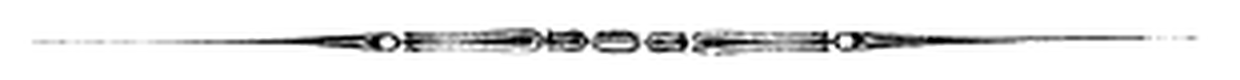
\includegraphics[width=0.48\linewidth]{assets/PA01_title_ornament_presentation_4x.png}
\end{center}

\noteid{GTH-A13 (PA20, final printer's ornament).} The final ornament is not approximated with generic TeX glyphs. A raw crop and a conservative presentation derivative are packaged. The raw source image is 575 by 741 pixels. The half-open crop box is \((x_0,y_0,x_1,y_1)=(245,360,375,395)\), yielding 130 by 35 pixels. The derivative applies grayscale preservation, full-range autocontrast, and 4x Lanczos resampling only, yielding 520 by 140 pixels. Hashes are:
\begin{quote}\ttfamily\footnotesize
raw: 664de1d2550bcccbb5db7117fcf091409c14b80958e1b9bacaf605bb5a5ce38e\\
derivative: b2969b2c39fb08c626b8683ec8a70203d0165ed30be85906f665e5a374d13fba
\end{quote}
\begin{center}
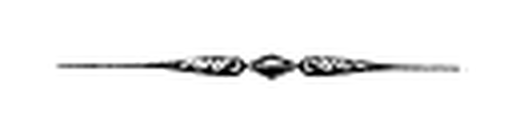
\includegraphics[width=0.24\linewidth]{assets/PA20_final_ornament_presentation_4x.png}
\end{center}


\noteid{GTH-A14 (PA08, \S 10, isolated definition of \(a_2\)).} The isolated definition prints
\[
a_2=-\frac{\pi^{2}}{a_1+2\lambda_1 i\pi},
\]
with a minus sign. The full iterative system later on the same page prints the corresponding definition with a positive numerator. Both local readings are retained in the diplomatic German and English bodies. The later positive form may indicate that the isolated minus is a typographical error, but no silent emendation is made.

\noteid{GTH-A15 (PA08, \S 10, isolated second transformation equation).} In the equation immediately following the isolated definition of \(a_2,b_2\), the printed left-hand side is \(\Theta(a,b)\), not \(\Theta(a_1,b_1)\). The subsequent full iterative system does print \(\Theta(a_1,b_1)\) at the corresponding stage. The diplomatic bodies preserve this local inconsistency; \(\Theta(a_1,b_1)\) is the contextually expected mathematical reading.

\noteid{GTH-A16 (PA11, \S 14, parameterization of \(\delta\)).} The final equality is printed with vertical delimiters:
\[
\delta=\delta_1+\gamma_1\delta_1(\alpha_1-\beta_1)
=\alpha_1\delta_1\lvert\gamma_1+\delta_1\rvert.
\]
The preceding \(\beta\)-line visibly uses braces, so the delimiter distinction is not normalized. The bars are reproduced diplomatically without imposing an interpretation beyond the printed glyphs.

\noteid{GTH-A17 (PA14, formula 18).} Formula 18 prints the prefactor denominator \(\varphi(2\alpha,\beta)\). The derivation immediately above ends with \(\varphi(2\alpha,\gamma)\), so \(\gamma\) is the mathematically motivated correction. The diplomatic bodies retain the printed \(\beta\); the probable correction is recorded only here.

\noteid{GTH-A18 (PA16, derived value of \(c\) before formula 19).} The source line reads
\[
2\sqrt{\gamma}\,e^{\gamma i\pi(2\beta+2-\delta)/4}=c\varphi(\alpha,2\gamma),
\]
with no minus sign in the exponent. Formula 19 immediately below also carries the positive exponent. Both monolingual bodies now preserve that reading.

\section*{4. Formula, figure, and layout policy}

All mathematical expressions are encoded as editable TeX. There are no authorial tables or diagrams. The non-formula graphical elements are the two title-page ornaments and the final printer's ornament, handled under GTH-A12--A13. The five repaired source-fidelity readings are documented under GTH-A14--A18. Lineation and page makeup are not reproduced as a facsimile; paragraph order, section sequence, equation labels, formula membership, and the relative order of all visible authorial elements are preserved. Page-unit anchors permit audit back to each physical witness.

\section*{5. Build and QA statement}

The three PDFs are built with pdfTeX under a fixed \texttt{SOURCE\_DATE\_EPOCH}, omitted creation dates, and fixed trailer identifiers. Clean rebuilds are byte-identical. Automated checks cover TeX failure, box warnings, PDF page counts, text extraction, source-anchor presence, German/English display-math parity, ZIP integrity, and SHA-256 manifests. Rendered contact sheets were visually inspected for clipping, overlap, broken glyphs, missing equations, and ornament placement. The machine-readable audit files in \texttt{05\_audit/} carry the detailed results.

\section*{6. Bibliographic identification}

Gordan, P. (1863). \textit{Ueber die Transformation der Thetafunctionen}. Giessen: Druck von Wilhelm Keller.

\end{document}
